% Created 2022-11-10 jue 23:25
% Intended LaTeX compiler: pdflatex
\documentclass[12pt]{article}
\usepackage[utf8]{inputenc}
\usepackage[T1]{fontenc}
\usepackage{graphicx}
\usepackage{grffile}
\usepackage{longtable}
\usepackage{wrapfig}
\usepackage{rotating}
\usepackage[normalem]{ulem}
\usepackage{amsmath}
\usepackage{textcomp}
\usepackage{amssymb}
\usepackage{capt-of}
\usepackage{hyperref}
\usepackage[spanish]{babel}
\usepackage{graphicx,geometry}
\geometry{ a4paper, left=1in, right=1in, top=1in, bottom=1in }
\renewcommand\familydefault{\sfdefault}
\usepackage{sectsty}
\sectionfont{\normalfont\Large }
\subsectionfont{\normalfont}
\usepackage{tabularx}
\usepackage{listings}
\lstdefinestyle{mystyle}{
numbers=left,
showspaces=false,
frame=single,
showspaces=false,
showstringspaces=false,
showtabs=false,
numberstyle=\tiny,
aboveskip=\parskip
}
\lstset{
style=mystyle,
literate={á}{{\'a}}1
{é}{{\'e}}1
{í}{{\'{\i}}}1
{ó}{{\'o}}1
{ú}{{\'u}}1
{Á}{{\'A}}1
{É}{{\'E}}1
{Í}{{\'I}}1
{Ó}{{\'O}}1
{Ú}{{\'U}}1
{ü}{{\"u}}1
{Ü}{{\"U}}1
{ñ}{{\~n}}1
{Ñ}{{\~N}}1
{¿}{{?``}}1
{¡}{{!``}}1
}
\makeatletter
\usepackage{fancyhdr}
\pagestyle{fancy}
\usepackage{mdframed}
\BeforeBeginEnvironment{minted}{\begin{mdframed}}
\AfterEndEnvironment{minted}{\end{mdframed}}
\author{Luis Eduardo Galindo Amaya (1274895)}
\date{09-11-2022}
\title{Organización de las Computadoras}
\hypersetup{
 pdfauthor={Luis Eduardo Galindo Amaya (1274895)},
 pdftitle={Organización de las Computadoras},
 pdfkeywords={},
 pdfsubject={},
 pdfcreator={Emacs 26.3 (Org mode 9.1.9)}, 
 pdflang={Spanish}}
\begin{document}



\newcommand{\docente}{Arturo Arreola Alvarez}
\newcommand{\asignatura}{Organización de Computadoras (331)}
\newcommand{\semestre}{2022-2}

\newcommand{\miportada}[1]{
	\begin{titlepage}
		\vspace*{0.75in}
		\begin{flushleft}
			\sffamily
			\large #1       \\
			\Huge 
            \@title         \\
			\hrulefill
			\vspace{0.25in} \\
			\Large \@author \\
			\vspace*{\fill}
            
\includegraphics[width=\textwidth]{../includes/filler.png} \\
			\vspace*{\fill}
			\large
			\begin{tabular}{|l|l|}
              \hline
			  Asignatura & \asignatura \\
			  Docente    & \docente    \\
			  Fecha      & \@date      \\
              \hline
			\end{tabular}
		\end{flushleft}
	\end{titlepage}
}

\miportada{ Notas II }

\fancyhf{}
\lhead{ \asignatura }
\rhead{ \semestre }
\rfoot{Página \thepage}

\setlength\parindent{0pt}   % eliminar el intentado
\setlength{\parskip}{1.2em}
\maketitle
\begin{figure}[htbp]
\centering
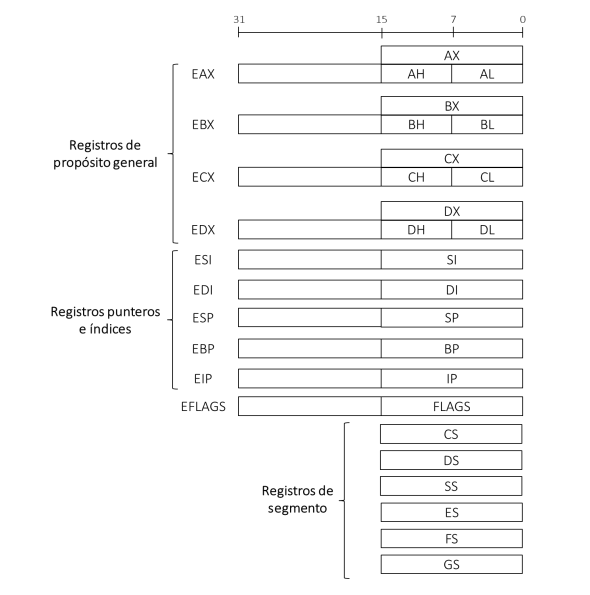
\includegraphics[width=.9\linewidth]{img/registros.png}
\caption{Registros del procesador}
\end{figure}

\section*{Contador De Programa (PC)}
\label{sec:orge46cac3}
El registro más importante es el Contador de programa (PC),
que apunta a la siguiente instrucción que se buscará para su
ejecución.

\section*{Registro De Propósito General}
\label{sec:orge1976f8}
\begin{itemize}
\item son 4 registros de 32 bits, EAX, EBX, ECX y EDX.
\item Son considerados de propósito general, pero tienen algunas funciones específicas.
\begin{description}
\item[{EAX}] El registro de aritmética principal.
\item[{EBX}] Para almacenar punteros a memoria.
\item[{ECX}] Bucles
\item[{EDX}] Se utiliza para multiplicacion y division
\end{description}
\end{itemize}

\subsection*{Partes Del Registro}
\label{sec:org4d957f3}
cada registro de proposito general esta dividido en cuatro secciones, en el caso del registro EAX, EAX, AX, AH y AL.

\begin{description}
\item[{EAX}] es el registro completo de 32 bits
\begin{description}
\item[{AX}] es la mitad del registro EAX (32 bits)
\begin{description}
\item[{AH}] es la mitad superior del registro AX (8 bits)
\item[{AL}] es la mitad inferior del registro AX (8 bits)
\end{description}
\end{description}
\end{description}

Podemos interpretar esto como una jerarquía de acceso al registro, no podemos pasar datos entre los registros si no son del mismo tamaño. Por ejemplo no podemos copiar el valor de \texttt{BX} en \texttt{EAX} porque \texttt{BX} es de 16 bits y \texttt{EAX} es de 32, pero si podemos pasar los valores de \texttt{EBX} a \texttt{EAX}, por lo tanto si queremos pasar un valor de un registro mas pequeño a uno mas grande tendremos que mover copiar el valor a un registro del mismo tamaño: 

\lstset{language=nasm,label= ,caption= ,captionpos=b,numbers=none,style=mystyle}
\begin{lstlisting}
;; esto no funciona
    mov eax, bx            

;; esto si funciona
;; aseguramos que el registro este vació 
    mov eax, 0               
    mov ax, bx
\end{lstlisting}

es importante entender que podemos ver el registro como un solo valor unico o como un valor con multiples partes para esto imaginemos la siguiente situacion, queremos representar un punto con sus coordenadas (cada una con una variable de 8 bits) : 

\lstset{language=nasm,label= ,caption= ,captionpos=b,numbers=none,style=mystyle}
\begin{lstlisting}
;; VALOR_X:  36 0010'0100
;; VALOR_Y: 127 0111'1111

    mov al, VALOR_X
    mov ah, VALOR_Y
\end{lstlisting}

como cada variables es de 8 bits en total esta estructura ocupa 16 bits de memoria, por lo que podemos ponerla en el registro \texttt{AX} sin problemas y así unimos dos intrucciones en una: 

\lstset{language=nasm,label= ,caption= ,captionpos=b,numbers=none,style=mystyle}
\begin{lstlisting}
;;  VALOR_X:    36            0010'0100
;;  VALOR_Y:   127            0111'1111
;; VALOR_YX: 32548  0111'1111'0010'0100

    mov aex, VALOR_YX
\end{lstlisting}

\section*{Registros De Punteros}
\label{sec:org34d843a}
\begin{itemize}
\item Contienen un registro de 16 bits en su parte menos significativa.
\item son 4 registros de 32 bits: 
\begin{description}
\item[{ESI y EDI}] se utilizan para almacenar punteros a memoria, especialmente para operaciones con cadenas
\item[{ESP}] Manipulación de la pila
\item[{EBP}] Apuntador a la pila
\item[{EIP}] Apuntador de instrucción
\end{description}
\end{itemize}

\section*{Registros De Segmentos}
\label{sec:org908bbfa}
\begin{itemize}
\item No se pueden separar.
\item Todos son de 16 bits.
\begin{description}
\item[{CS}] Segmento de código.
\item[{DS}] Segmento de datos.
\item[{SS}] Segmento de pila
\item[{ES, FS y GS}] Segmentos extra.
\end{description}
\end{itemize}

\section*{Registro De Banderas}
\label{sec:org3199ddc}
\subsection*{Registros de banderas}
\label{sec:org0c3e2d0}
\begin{itemize}
\item Registro de 32 bits.
\item Bits 18 al 31 están reservados.
\item Bits 0 al 11 bits de banderas.
\item Indica la condición actual del procesador.
\item Contiene información de la última operación aritmética
\end{itemize}

\subsection*{Banderas}
\label{sec:org76659a0}
\begin{description}
\item[{Signo de la operacion (S)}] 0 positivo y 1 negativo
\item[{Parieradad (P)}] 0 impar, 1 par
\item[{Interrupciones (I)}] 0 activadas, 1 desactivadas
\item[{sobreflujo (O)}] bit de sobreflujo
\end{description}

\subsection*{Significado De Cada Registro}
\label{sec:org196114b}
\begin{center}
\begin{tabular}{|r|l|l|}
\hline
POS & Abreviacions & Significado\\
\hline
0 & C & Acarreo\\
1 &  & \\
2 & P & Paridad\\
3 &  & \\
4 & A & Acarreo auxiliar\\
5 &  & \\
6 & Z & Cero\\
7 & S & Signo\\
8 & T & Bandera trampa\\
9 & I & Habilitar interrupciones\\
10 & D & Bandera de dirección\\
11 & O & Sobreflujo\\
12 & IO PL & -\\
13 & IO PL & -\\
14 & NT & -\\
15 &  & \\
16 & RF & \\
17 & VM & \\
\hline
18-31 & RESERVADOS & \\
\hline
\end{tabular}
\end{center}

\section*{Modos De Redireccionamiento}
\label{sec:org202ee26}
\subsection*{Caracteristicas}
\label{sec:org61a6285}
\begin{description}
\item[{Deplazamiento}] que se se suma un valor fijo a \texttt{DS}\footnote{Segmento de datos.}
\item[{Base}] que tiene un registro para la posicion
\item[{Indice}] que tiene un registro que puede cambiar su valor
\item[{Índice escalado}] es un registro que se multiplica por el tamaño del tipo de dato que se desea conocer
\end{description}

\subsection*{Tabla De Redireccionamiento Completa}
\label{sec:orgdd0e2de}
\begin{center}
\begin{tabular}{|l|l|}
\hline
Inmediato & \texttt{MOV EAX, 0x12345678}\\
\hline
Registro & \texttt{MOV EBP, EAX}\\
\hline
Desplazamiento & \texttt{MOV EAX, [12]}\\
\hline
Base & \texttt{MOV EAX, [EBX]}\\
\hline
Base con desplazamiento & \texttt{MOV EAX, [EBX+E7027193]}\\
 & \texttt{MOV [ESP–5],AH}\\
\hline
Base con índice & \texttt{MOV EAX, [ECX+EBP]}\\
 & \texttt{MOV word [EDI+ESI], F5}\\
\hline
Base con índice y desplazamiento & \texttt{MOV EAX, [ECX+EBP+2F19]}\\
 & \texttt{MOV [ESP][ECX][4B024], AH}\\
 & \texttt{MOV EDX, [EBP+EBX-E02719]}\\
\hline
Índice escalado & \texttt{MOV EAX, [ECX*4]}\\
 & \texttt{MOV [EBP*2], AH}\\
\hline
Índice escalado y desplazamiento & \texttt{MOV EAX, [5][ECX*4]}\\
 & \texttt{MOV word[EDI*8+1F3], 1B}\\
\hline
Base con índice escalado & \texttt{MOV EAX, [EBP+ECX*4]}\\
 & \texttt{MOV [EDX*2+EBP], CH}\\
\hline
Base con índice escalado y Con & \texttt{MOV [38][ECX+EBP*4], AX}\\
desplazamiento & \texttt{MOV [2A][EDX*2+EBP], CH}\\
\hline
\end{tabular}
\end{center}

\section*{Conjunto De Instrucciones}
\label{sec:org92f8d35}
\begin{center}
\begin{tabular}{|l|l|}
\hline
Instrucción & Descripción\\
\hline
\texttt{XCHG} & Intercambia valores entre una dos registros del\\
 & mismo tamaño o una posición de memoria y\\
 & un registro.\\
\hline
\texttt{IN} & Lee un dato de un dispositivo de E/S y lo\\
 & almacena en el acumulador.\\
\hline
\texttt{OUT} & Transfiere un dato del acumulador a un puerto\\
 & de E/S.\\
\hline
\texttt{LAHF} & Carga el byte menos significativo del registro\\
 & de banderas en AH\\
\hline
\texttt{SAHF} & Almacena el valor de AH en el byte menos\\
 & significativo en EFLAGS.\\
\hline
\texttt{LEA} & Guarda en el primer operando la dirección\\
 & efectiva del segundo operando.\\
\hline
 & \\
 & \textbf{INSTRUCCIONES DE LA PILA}\\
\hline
Instrucciones & Descripción\\
\hline
\texttt{PUSH} & Inserta un dato de 16/32 bits a la pila\\
\hline
\texttt{POP} & Remueve un dato de 16/32 bits de la pila\\
\hline
\texttt{PUSHF} & mete los bits 0-15 del registro de banderas a la pila\\
\hline
\texttt{POPF} & remueve 2 bytes de la pila y los almacena en EFLAGS.\\
\hline
\texttt{PUSHFD} & PUSHFD mete los bits 0-31 del registro de banderas a\\
 & la pila\\
\hline
\texttt{POPFD} & POPF remueve 4 bytes de la pila y los almacena\\
 & en EFLAGS\\
\hline
\end{tabular}
\end{center}

\pagebreak

\section*{Pila}
\label{sec:org9867318}
\subsection*{Generalidades de la pila}
\label{sec:org3f49e45}
La pila guarda los valores de manera decreciente por lo tanto los valores agregados a la pila al final obtendran posiciones mas significativas:

\begin{figure}[htbp]
\centering
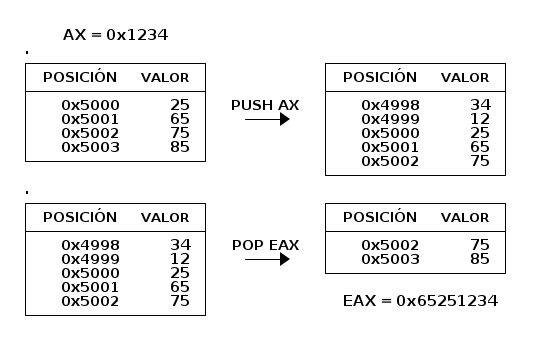
\includegraphics[width=14cm]{img/pila.png}
\caption{Comportamiento de la pila}
\end{figure}


\subsection*{PUSH}
\label{sec:orgf703ee4}
\begin{description}
\item[{16 bits}] push con un registro de 16 bits (\texttt{AX}, \texttt{BX}, \texttt{CX}, \texttt{DX})
\item[{32 bits}] push con un registro de 32 bits (\texttt{EAX}, \texttt{EBX}, \texttt{ECX}, \texttt{EDX})
\end{description}

\subsubsection*{Otras formas de PUSH}
\label{sec:org963eecc}
\begin{description}
\item[{\texttt{PUSH WORD 4567h}}] Inserta a la pila el valor inmediato \texttt{4567h}.
\item[{\texttt{PUSH DWORD 154567h}}] Inserta a la pila el valor inmediato \texttt{154567h}.
\item[{\texttt{PUSH WORD[ECX]}}] Inserta a la pila el valor almacenado en \texttt{Mem[ECX]}.
\item[{\texttt{PUSH DWORD[ECX+ESI*4]}}] Inserta a la pila el valor almacenado en \texttt{Mem[ECX+ESI*4]}.
\end{description}

\noindent\rule{\textwidth}{0.5pt}

\subsection*{POP}
\label{sec:org082b76b}
\begin{description}
\item[{16 bits}] pop con un registro de 16 bits (\texttt{AX}, \texttt{BX}, \texttt{CX}, \texttt{DX})
\item[{32 bits}] pop con un registro de 32 bits (\texttt{EAX}, \texttt{EBX}, \texttt{ECX}, \texttt{EDX})
\end{description}

\subsubsection*{Otras formas de POP}
\label{sec:org3d65dc5}
\begin{description}
\item[{\texttt{POP WORD[ECX]}}] Remueve de la pila 16 bits y los almacena en \texttt{Mem[ECX]}.
\item[{\texttt{PUSH DWORD[ECX+ESI*4]}}] Remueve de la pila 32 bits y los almacena en \texttt{Mem[ECX + ESI*4]}.
\end{description}

\noindent\rule{\textwidth}{0.5pt}

\section*{Operaciones Aritméticas}
\label{sec:orgf3997c0}
\begin{center}
\begin{tabular}{|l|l|}
\hline
Instrucción & Descripción\\
\hline
\texttt{ADD} & Suma los operandos y almacena el resultado en el\\
 & primer operando.\\
\hline
\texttt{ADC} & Realiza la operación de suma entre los operandos,\\
 & sumándole el bit de acarreo del registro de\\
 & banderas (suma de 64 bits)\\
\hline
\texttt{INC} & Incrementa en 1 el operando\\
\hline
\texttt{SUB} & Resta los operandos y almacena el resultado en el\\
 & primer operando\\
\hline
\texttt{SBB} & Realiza la operación de resta entre los operandos,\\
 & restando el bit de acarreo del registro de\\
 & banderas (resta de 64 bits).\\
\hline
\texttt{DEC} & Decrementa en 1 el operando.\\
\hline
\texttt{TEST} & Realiza una operación AND entre dos operandos y\\
 & actualiza el estado del registro de banderas\\
\hline
\end{tabular}
\end{center}

\subsection*{Multiplicación (\texttt{MUL})}
\label{sec:orgec1c8b6}
Multiplica el operando por AL, AX o EAX.
\begin{itemize}
\item \texttt{MUL BL} se puede traducir como \texttt{AX = AL*BL}
\item \texttt{MUL DI} se puede traducir como \texttt{DX:AX = AX*DI}
\item \texttt{MUL ECX} se puede traducir como \texttt{EDX:EAX = EAX*ECX}
\item \texttt{MUL Word[EBP]} se puede traducir como \texttt{DX:AX = AX*Mem[EBP]}
\end{itemize}

\subsection*{Multiplicación (\texttt{IMUL})}
\label{sec:org83f1258}
IMUL reg / IMUL mem
\begin{itemize}
\item \texttt{IMUL BL} puede traducirse como \texttt{AX = AL*BL}
\item \texttt{IMUL DI} puede traducirse como \texttt{DX:AX = AX*DI}
\item \texttt{IMUL ECX} puede traducirse como \texttt{EDX:EAX = EAX*ECX}
\item \texttt{IMUL Word[EBP]} puede traducirse como \texttt{DX:AX = AX*Mem[EBP]}
\end{itemize}

\subsection*{División de 8 bits (\texttt{DIV} e \texttt{IDIV})}
\label{sec:orgbfc98d8}
\begin{itemize}
\item Coloca el resulado de la division de \texttt{AL} y el modulo de la operacion en \texttt{AH}.
\item \texttt{DIV BL} se puede traducir como \texttt{AL = AX/BL} y \texttt{AH = AX\%BL}
\item \texttt{IDIV CL} se puede traducir como \texttt{AL = AX/CL} y \texttt{AH = AX\%CL}
\item \texttt{DIV byte[ESI]} se puede traducir como \texttt{AL = AX/Mem[ESI]} y \texttt{AH = AX\%Mem[ESI]}
\end{itemize}

\subsection*{División de 16 bits (\texttt{DIV} e \texttt{IDIV})}
\label{sec:orgcb111ac}
\begin{itemize}
\item Coloca el resulado de la division de \texttt{EAX} y el modulo de la operacion en \texttt{EDX}.
\item \texttt{DIV EBX} se puede traducir como \texttt{EAX = EDX:EAX/EBX}
\item \texttt{DIV ECX} se puede traducir como \texttt{EAX = EDX:EAX/ECX}
\item \texttt{DIV dword[ESI]} se puede traducir como \texttt{EAX=EDX:EAX/Mem[ESI]}
\end{itemize}

\pagebreak

\section*{Instrucciones Lógicas}
\label{sec:org256d8b2}
\begin{description}
\item[{OR}] Se activa cuando al menos una variable está activa.
\end{description}
\lstset{language=nasm,label= ,caption= ,captionpos=b,numbers=none,style=mystyle}
\begin{lstlisting}
;; Ejemplo de OR

    MOV AL, 10001010b
    OR AL, 01001010b            ;11001010b

;; 10001010b
;; 01001010b  
;; ---------
;; 11001010b

\end{lstlisting}
\begin{description}
\item[{AND}] Solo se activa cuando ambas variables estan activas
\end{description}
\lstset{language=nasm,label= ,caption= ,captionpos=b,numbers=none,style=mystyle}
\begin{lstlisting}
;; Ejemplo de AND

    MOV AL, 10001010b
    AND AL, 01001010b            ;00001010b

;; 10001010b
;; 01001010b  
;; ---------
;; 00001010b

\end{lstlisting}
\begin{description}
\item[{XOR}] Se activa cuando solo una variables está activa
\end{description}
\lstset{language=nasm,label= ,caption= ,captionpos=b,numbers=none,style=mystyle}
\begin{lstlisting}
;; Ejemplo de AND

    MOV AL, 10001010b
    XOR AL, 01001010b            ;11000000b

;; 10001010b
;; 01001010b  
;; ---------
;; 11000000b

\end{lstlisting}

\subsection*{Tablas de verdad}
\label{sec:orgc3559d7}
\begin{center}
\begin{tabular}{|rr|r|r|r|}
\hline
VAR X & VAR Y & OR & AND & XOR\\
\hline
0 & 0 & 0 & 0 & 0\\
0 & 1 & 1 & 0 & 1\\
1 & 0 & 1 & 0 & 1\\
1 & 1 & 1 & 1 & 0\\
\hline
\end{tabular}
\end{center}

\section*{Corrimientos}
\label{sec:org62faf06}
Las instrucciones de corrimiento posicionan o mueven números a la izquierda o a la derecha dentro de un registro o localidad de memoria, excepto los registros de segmento.

\begin{center}
\begin{tabular}{|l|l|l|}
\hline
Instrucción & Descripción & Valor En El Carry\\
\hline
\texttt{SHL} & shift a la izquierda & El valor mas a la izquierda\\
\hline
\texttt{SHR} & shift a la derecha & El valor mas a la Derecha\\
\hline
\end{tabular}
\end{center}

\section*{Corrimientos}
\label{sec:orga2084b1}
Las instrucciones de corrimiento posicionan o mueven números a la izquierda o a la derecha dentro de un registro o localidad de memoria, excepto los registros de segmento.

\begin{center}
\begin{tabular}{|l|l|l|}
\hline
Instrucción & Descripción & Valor En El Carry\\
\hline
\texttt{SHL} & shift a la izquierda & El valor mas a la izquierda\\
\hline
\texttt{SHR} & shift a la derecha & El valor mas a la Derecha\\
\hline
\end{tabular}
\end{center}

\section*{Control de Programa}
\label{sec:org814f672}
\begin{description}
\item[{\texttt{JMP}}] Salto incondicional.
\item[{\texttt{LOOP}}] decrementa el valor de \texttt{CX} hasta llegar a 0.
\item[{\texttt{LOOPE}}] Salta si \texttt{CX} es diferente de cero mientras una condición de igual existe (Z=1).
\item[{\texttt{LOOPNE}}] Salta si CX es diferente de cero mientras una condición de no igual exista (Z=0).
\item[{\texttt{CALL}}] Realiza un salto hacia un procedimiento. Guarda en la pila la dirección de retorno.
\item[{\texttt{RET}}] Realiza un salto hacia la dirección de retorno, sacándola de la pila.
\item[{\texttt{CMP}}] Realiza una resta entre los operandos sin modificarlos.
\end{description}

\begin{center}
\begin{tabular}{|l|l|}
\hline
Instrucción & Banderas que comprueba\\
\hline
JC & C = 1\\
JNC & C = 0\\
JZ, JE & Z = 1\\
JNZ, JNE & Z = 0\\
JS & S = 1\\
JNS & S = 0\\
JO & O = 1\\
JNO & O = 0\\
JP, JPE & P = 1\\
JNP, JPO & P = 0\\
\hline
\end{tabular}
\end{center}

\subsection*{Comparaciones}
\label{sec:org335fdca}
\subsubsection*{Números sin signo}
\label{sec:orgc081fbe}
\begin{center}
\begin{tabular}{|l|l|l|}
\hline
Instrucción & Banderas que comprueban & Descripción\\
\hline
JA, JNBE & CF = 0 y ZF = 0 & Salta si es mayor\\
JAE, JNB,JNC & CF = 0 & Salta si es mayor o igual\\
JB, JNAE, JC & CF = 1 & Salta si es menor\\
JBE, JNA & CF = 1 ó ZF = 1 & Salta si es menor o igual\\
\hline
\end{tabular}
\end{center}


\subsubsection*{Números con signo}
\label{sec:org37c4a04}
\begin{center}
\begin{tabular}{|l|l|l|}
\hline
Instrucción & Banderas que comprueba & Descripción\\
\hline
JG, JNLE & SF = OF y ZF = 0 & Salta si es mayor\\
JGE & SF = OF & Salta si es mayor o igual\\
JL, JNGE & SF ≠ OF & Salta si es menor\\
JLE, JNG & SF ≠ OF ó ZF = 1 & Salta si es menor o igual\\
\hline
\end{tabular}
\end{center}
\end{document}
